% Copyright 2023 Andy Casey (Monash) and friends
% TeX magic by David Hogg (NYU)

\documentclass[modern]{aastex631}
\usepackage[utf8]{inputenc}
\usepackage{amsmath}
\usepackage{MnSymbol}
\usepackage{rotating}

\renewcommand{\twocolumngrid}{}
\addtolength{\topmargin}{-0.35in}
\addtolength{\textheight}{0.6in}
\setlength{\parindent}{3.5ex}
\renewcommand{\paragraph}[1]{\medskip\par\noindent\textbf{#1}~---}

% figure setup
\usepackage{graphicx}
\usepackage{xcolor}
\usepackage[framemethod=tikz]{mdframed}
\usetikzlibrary{shadows}
\definecolor{captiongray}{HTML}{555555}
\mdfsetup{%
innertopmargin=2ex,
innerbottommargin=1.8ex,
linecolor=captiongray,
linewidth=0.5pt,
roundcorner=1pt,
shadow=false,
}
\newlength{\figurewidth}
\setlength{\figurewidth}{0.75\textwidth}

\newcommand{\norm}[1]{\left\lVert#1\right\rVert}

% Other possible titles
%\newcommand{\chosentitle}{Constrained linear models for stellar spectroscopy}
%\newcommand{\chosentitle}{Constrained linear absorption models for stellar spectroscopy}
%\newcommand{\chosentitle}{The Unreasonable Effectiveness of Linear Models in Stellar Spectroscopy}
%\newcommand{\chosentitle}{Stellar continuum modelling}
\newcommand{\chosentitle}{Constrained linear absorption models for stellar spectroscopy}

\shorttitle{\chosentitle}
\shortauthors{Casey}
\newcommand{\documentname}{\textsl{Article}}
\newcommand{\sectionname}{Section}

\newcommand{\project}[1]{\textit{#1}}
\renewcommand{\vec}[1]{\mathbf{#1}}
\newcommand{\vectheta}{\boldsymbol{\theta}}
\newcommand{\vecalpha}{\boldsymbol{\alpha}}
\newcommand{\vecbeta}{\boldsymbol{\beta}}
\newcommand{\vecgamma}{\boldsymbol{\gamma}}
\newcommand{\vecW}{\mathbf{W}} % stellar line absorption basis weights
\newcommand{\vecF}{\mathbf{F}} % stellar line absorption basis vectors
\newcommand{\vecG}{\mathbf{G}} % telluric line absorption basis vectors
\newcommand{\vecH}{\mathbf{H}} % continuum basis vectors
\newcommand{\vecX}{\mathbf{X}}

\newcommand{\hadamard}{\odot}
\newcommand{\apogee}{\project{APOGEE}}
\newcommand{\boss}{\project{BOSS}}
\newcommand{\sdss}{\project{SDSS}}
\newcommand{\eso}{\project{ESO}}
\newcommand{\harps}{\project{HARPS}}

\newcommand{\unit}[1]{\mathrm{#1}}
\newcommand{\mps}{\unit{m\,s^{-1}}}
\newcommand{\kmps}{\unit{km\,s^{-1}}}
\newcommand*{\transpose}{^{\mkern-1.5mu\mathsf{T}}}


\definecolor{tab:blue}{HTML}{1170aa}
\definecolor{tab:red}{HTML}{d1615d}
\newcommand{\todo}[1]{\textcolor{tab:red}{#1}}

\newcommand{\ajw}[1]{\textbf{#1}}

\sloppy\sloppypar\raggedbottom\frenchspacing
\begin{document}

\title{\chosentitle}

\author[0000-0003-0174-0564]{Andrew R. Casey}
\affiliation{School of Physics \& Astronomy, Monash University, Australia}
\affiliation{Centre of Excellence for Astrophysics in Three Dimensions (ASTRO-3D)}
\affiliation{Center for Computational Astrophysics, Flatiron Institute, a division of the Simons Foundation}

\author{friends}
%\author[0000-0003-2866-9403]{David W. Hogg}
%\affiliation{Center for Cosmology and Particle Physics, Department of Physics, New York University}
%\affiliation{Max-Planck-Institut f\"ur Astronomie, Heidelberg}
%\affiliation{Center for Computational Astrophysics, Flatiron Institute, a division of the Simons Foundation}


\begin{abstract}\noindent
Forward modelling stellar spectra usually requires a spectral synthesis code, or a non-linear interpolator \ajw{emulator?} constructed from a curated training set.
These approaches require pre-processing steps (e.g., continuum rectification) which, when performed separately, can bias scientific inferences.
Here we describe a constrained \emph{linear} model that can fit radial velocity, rotational broadening, stellar absorption, telluric transmission, the joint continuum-instrument response.
Stellar absorption and telluric transmission are each modelled by factorizing a grid of rectified theoretical spectra into two non-negative matrices: basis weights and basis vectors.
The non-negativity constraint ensures that basis vectors are strictly additive. \ajw{consider dropping or rewording this sentence}
The joint continuum-instrument response is modelled with a Fourier basis.
Together this set of bases represents an effective linear model for stellar spectroscopy. \ajw{Could potentially be made more precise? see note at top of intro.}
The model requires no initial guess or tuning, and the linearity ensures that inference is convex, stable, and fast.
This model allows us to reliably fit nuisances (e.g., tellurics, continuum, radial velocity, rotational or macroscopic broadening), without any prior knowledge about the fundamental stellar properties.
We demonstrate our method by fitting \eso/\harps\ high-resolution echelle spectra of BAFGKM-type stars.
From repeat observations of $\alpha$-Centauri A we show that our approach yields continuum estimates that are consistent to 0.2\% at S/N $\sim$ 100, and better than 0.5\% at S/N $\sim$ 30.
\end{abstract}

% for S/N > 100, 1-sigma scatter is 0.22%
% for S/N > 50, 1-sigma scatter is 0.35%
% for S/N > 30, 1-sigma scatter is 0.46%

\keywords{\todo{Some --- keywords --- here}}

\section*{}\noindent\todo{
Known issues to resolve before submission:\\
- Update HARPS fits to use blaze-corrected flux (only AB-type stars use it now)\\
- In the "alpha Cen A" sample, sometimes they accidentally observed alpha Cen B and didn't realise! Maybe better to use a different star?\\
- Add citations\\
- Update red text.
}


\clearpage
\section{Introduction}\label{sec:intro}

\ajw{
The abstract mostly talks about the model, and the introduction mostly talks about continuum normalization.  Would be good to more explcitly link, maybe.
I also think that it would be good to more precisely state what about this model is good.
Something like: it characterizes the set of all possible spectra in many few parameters than other d-d models, while still expcluding enough unphysical ``spectra'' (thanks to NN constraint) that you can, e.g. project onto it to separate spectrum from continuum (or use it for param estimation).
}

Continuum normalization\footnote{Or continuum rectification, as it was historically described.} is often required before estimating stellar parameters and chemical abundances, because those quantities are inferred from line strengths that are measured \emph{relative} to the continuum.
\ajw{Would be good to say that the more fundemental reason is that modelling the continuum (mostly intrumental but also stellar) is hard, and the separation is feasible for most stars.}
The practice of continuum rectification is ripe with subjectivity, in part for justified historical reasons. Often a consistent procedure is more useful than an abstract \ajw{maybe reword} one, so people tend to stick with what they know, and that subjectivity is inherited by graduate students. While there is general agreement in the literature that is important to achieve consistent continuum normalization, there is no apparent consensus on how it should be done.\\

The literature describes a variety of rectification strategies used to achieve different goals. Classical spectroscopists might make some coarse estimate of the continuum for the spectrum, and locally refine that estimate for every absorption line of interest. This process is often done by hand,\footnote{Albeit they are often experienced hands. See \citet{Bensby:2014}: \quote{`\emph{more than 300\,000 equivalent widths were measured by (the first author's right) hand}'}.} although some graphical user interface tools exist to streamline the process and improve reproducibility. This approach usually restricts the spectroscopist to only measuring strengths of what are believed to be isolated lines: atomic transitions that are not contaminated by neighbouring lines or molecular bands. In contrast, industrial spectroscopists often have a different objective: one where they solely for a \emph{consistent} continuum normalization procedure. In those situations the process does not have claim to deliver the true continuum, but it should deliver a \emph{pseudo}-continuum that is consistent for stars of similar stellar parameters and signal-to-noise (S/N) ratios.\\

Fitting the continuum correctly requires you to know where there is absorption. But knowing where there is line absorption requires you to (at least) know the stellar parameters \ajw{confused about this claim}. Without knowing the stellar parameters -- or having a good model for line absorption -- spectroscopists have developed various bespoke methods. A popular choice is to iteratively mask pixels in an asymmetric manner (so-called `sigma clipping') to exclude data points some chosen level below the current estimate of the continuum. This works well if the practictioner can confidently set the bounds on where to exclude data. However, those parameters would need to be different for a more metal-rich star, or for a spectrum with a low S/N ratio. Exactly how to specify the asymmetric clipping parameters comes down to experience.\\

An alternative is simply to mask all pixels except a carefully selected set of so-called `continuum pixels'. This is painstaking work to perform manually, but can be done by iteratively training data-driven models, or building masks from approximate line strengths computed from atomic properties. In either scenario, the set of continuum pixels is only valid for stars of a similar type and metallicity. In many cases there are simply \emph{no} continuum pixels (e.g., near a molecular absorption band in an M-dwarf). Some graphical tools exist to enable practictioners to select pseudo-continuum points to `anchor' some continuum fit (e.g., a spline, or through a rolling-pin analogy) which are useful if the practictioner wants full control over the continuum fit, or if the models are particularly poor at predicting continuum pixels.\\

We might simply consider what is the best continuum for every possible theoretical spectrum under comparison. When there are thousands of model spectra to compare with, then for each spectrum we can take the ratio of the data and the model, apply some averaging filter (e.g., moving mean or median) and take that as the pseudo-continuum. These kinds of approaches work remarkably well, despite the requirement of a (potentially very large) set of sufficiently similar model spectra, and the added computational expense.\\


In an ideal scenario the continuum is jointly fit with the stellar parameters. Unfortunately, predicting the emergent spectrum is usually expensive. In Section~\ref{sec:methods} we describe a family of methods to address these problems.
The methods we describe uses non-negative matrix factorization (NMF) to approximate line absorption and telluric transmission. NMF is a linear model to describe large non-negative matrix by two smaller matrices, both with non-negative elements. This non-negativity provides a very useful constraint that is applicable in many areas of astronomy (i.e., where things cannot physically be negative), but NMF has seen relatively little use in astronomy compared to other research areas, or other dimensionality reduction techniques. 
We describe data (Section~\ref{sec:experiments}) and experiments using this model, where the results are presented in Section~\ref{sec:results}. We discuss limitations and potential extensions of our work in Section~\ref{sec:discussion}, before concluding in Section~\ref{sec:conclusions}.\\

%The typical analysis procedure for this kind of spectra might involve selecting (by hand) pixels that do not appear to be obviously affected by line (or molecular) absorption, and fitting a smooth function to represent the continuum. This process would be repeated per-order, often ignoring the selection of pixels in the previous order (which overlaps in wavelength). A subsequent local continuum determination would be made for each line.


\section{Methods}\label{sec:methods}
\ajw{Weinberg does a thing where he has a table of every variable and what it is at the beginning of the methods.  It makes things much easier to skim, and I think it would work well here.}

We will assume a forward model that includes three components: one that represents continuum-normalized stellar absorption (e.g., molecular or atomic line absorption) \ajw{I think stellar lines   would be a better name for this, the relationship between actual absorption and lines is kinda subtle }; a second to describe telluric transmission; and a third to represent the smooth continuum.\footnote{In this work the `continuum' always refers to the joint continuum-instrument response. In many spectrographs these are different, but cannot be disentangled without extra work.} We will require all components to be linear models, which ensures that inference is stable and fast. In practice the linear models we construct seem sufficient to model stellar spectra for the purposes of continuum normalization and handling other nuisances.\\

% TODO: list explicit assumptions with hogg in person

Here we will describe the method in general before outlining the implementation details. We assume the data are a one-dimensional spectrum with $P$ pixels, where the $i$-th pixel has wavelength $\lambda_i$, flux $y_i$, and flux error $\sigma_{y_i}$ (with $1 \leq i \leq P$). The forward model for the flux in the $i$-th pixel can be expressed as the element-wise (Hadamard; $\hadamard$) multiplication of what we will describe as the stellar absorption model $f(\lambda_i; \vecalpha)$, the telluric transmission model $g(\lambda_i; \vecbeta)$, and the continuum-instrument response model $h(\lambda_i;\vecgamma)$
\begin{align}\label{eq:y}
    y_i &= f(\lambda_i;\vecalpha)\hadamard{}g(\lambda_i;\vecbeta)\hadamard{}h(\lambda_i;\vecgamma) + \mbox{noise}
\end{align}
where the components $f(...)$, $g(...)$, and $h(...)$ are defined below. Throughout this paper we fit in (natural) log-transformed data space $\vec{Y} = \log{\vec{y}}$ with the transformed variance in the $i$-th pixel
\ajw{you should probably say that C is the (diagonal) cov matrix}
\begin{eqnarray}
    \vec{C}_{ii} = \left(\frac{\sigma_{y,i}}{y_i} - \frac{\sigma_{y,i}^2}{2y_i^2} + \frac{2\sigma_{y,i}^3}{8y_i^3} - \frac{6\sigma_{y,i}^4}{24y_i^4}\right)^2
\end{eqnarray}
\noindent{}which is computed by taking a swiftly \ajw{?} Taylor series expansion. The log-transformation changes the element-wise product of three model components into the convenient summation:
\begin{align}
    \label{eq:log_y}
    \vec{Y} &= \log{f(\vec{\lambda}; \vecalpha)} + \log{g(\vec{\lambda};\vecbeta)} + \log{h(\vec{\lambda};\vecgamma)} \quad .
\end{align}\\

We now turn to defining each model component in detail.
The stellar absorption model $f(\lambda_i;\vecalpha)$ predicts \ajw{represents? corresponds to?} the rectified stellar line absorption at wavelength $\lambda_i$ given parameters $\vecalpha$. We construct the line absorption model $f(\lambda_i;\vecalpha)$ from a set of $N$ continuum-normalized theoretical spectra (each with $D$ fluxes) using non-negative matrix factorization (NMF).
The theoretical spectra used to construct the line absorption model do not have to have the same wavelength sampling and instrument line spread profile as the data, but at inference time there is a need to interpolate (or evaluate) the line absorption model to the $P$ observed wavelengths.\\

We refer to our $N \times D$ matrix of continuum-rectified theoretical stellar spectra as $\vec{S}$. This is a dense matrix: there are no entries of exactly zero, with many entries near 1 (no absorption). However, a small transformation to this matrix makes it extremely sparse. Numerous transformations are possible\footnote{Another sparse transformation is $1 - \vec{M}$, but this makes our resulting model non-linear.}, but for many reasons we chose to factorize the negative logarithm of $\vec{S}$ into two smaller matrices $\vec{W}_\star$ and $\vec{F}$ such that,
\begin{eqnarray}
    \label{eq:nmf}
    -\log\left({\vec{S}}\right) \approx \vec{W}_\star\transpose\vec{F}
\end{eqnarray}
where $\vec{W}_\star$\footnote{The star in $\vec{W}_\star$ differentiates it from the basis weights found from factorizing telluric spectra $\vec{W}_\earth$.} is a $K \times N$ matrix of \emph{basis weights}, where $K$ is the number of chosen basis vectors, and $\vec{F}$ is a $K \times D$ matrix of NMF \emph{basis vectors}. The factorization of $-\log{\vec{S}}$ into $\vec{W}_\star\transpose\vec{F}$ requires that all elements in $-\log\left({\vec{S}}\right)$, $\vec{W}_\star$, and $\vec{F}$ be non-negative. The number of basis components $K$ should be significantly smaller than both the number of input spectra $N$ and the number of pixels $D$ per spectrum.\\

The factorization of $-\log\left({\vec{S}}\right)$ into $\vec{W}_\star\transpose\vec{F}$ is reasonably fast and easy to compute given existing packages in modern programming languages. In general we found substantial improvements by initializing $\vec{F}$ with non-negative double singular value decomposition, where zeros were filled-in with the average of $-\log\left({\vec{S}}\right)$: this is the default behaviour in many packages. We found very similar looking basis vectors if we initialized from random values, but it took more training iterations. We found that factorizing $\vec{W}_\star\transpose\vec{F}$ by coordinate descent was substantially faster than using multiplicative updates, \todo{until reaching a plateau in reconstruction error, at which point we would iterate further using multiplicative updates.} The multiplicative update rules are appealing because they are convex, do not require many choices, and they can be efficiently iterated on a graphics card.\\


There are very few requirements of the theoretical spectral grid. There are no requirements on the number of dimensions (e.g., whether or not to include $[\alpha/\mathrm{Fe}]$, $[\mathrm{C/Fe}]$), and no strict requirements (see Section~\ref{sec:discussion}) on spacing between points. The only implicit requirement is that the theoretical spectra should approximately span the range of stars that you intend to fit. This is more of a recommendation than a requirement: in practice we found that a grid trained on theoretical spectra of A- to M-type stars was also sufficiently flexible to model many O-type stars, but there was structured residuals in the wings of hydrogen lines. For these reasons, we chose to include as many theoretical spectra as our memory constraints would allow.\footnote{If the number of spectra exceeds your memory constraints then there are numerous strategies available: you can use memory-mapped arrays, use lower precision float types, compute updates in batches, or simply skip every $n$th spectrum.}\\

We used the BOSZ spectral grid to construct basis vectors for a stellar line absorption model. This is a high-resolution ($\mathcal{R} \sim 300{,}000$) finely sampled theoretical grid computed using the \texttt{ATLAS9} code with \project{MARCS} spherical and plane-parallel models atmospheres. While the grid does include spectra for hotter stars computed with ATLAS atmospheres, we restricted ourselves to MARCS model atmospheres for this work. The grid spans a reasonably large range in stellar parameters, covers the complete wavelength range of the \eso/\harps\ instrument, and importantly it includes the theoretical continuum for each spectrum. We constructed a sparse kernel to convolve the rectified flux to the \eso/\harps\ spectral resolution of $\mathcal{R} \sim 115{,}000$, truncated the convolved spectra between 300-700\,nm, and clipped any rectified flux values exceeding 1 (e.g., emission lines) as they violate our NMF requirements. The matrix $\vec{S}$ includes all \todo{X} convolved BOSZ spectra, with \todo{N} pixels each, which we randomly shuffled at every iteration during factorization. We factorized this matrix into $K = 16$ basis vectors by coordinate descent for \todo{10,000} steps, \todo{and then X steps using multiplicative updates}. After training, the Frobenius loss, also known as the L2 reconstruction loss
\begin{eqnarray}
    L_2 = \norm{{\left(-\log{\vec{S}}\right) - \vec{W}_\star\transpose\vec{F}}}^2
\end{eqnarray}
\noindent{}was found to be \todo{X}. Figure~\ref{fig:schematic} shows some example basis vectors computed by this factorization, where it is somewhat striking that the basis vectors are identifiable by astrophysical mechanism, since no stellar parameters (or astrophysics of any kind) are included in the factorization process. For example, one basis vector just includes hydrogen lines. Another basis vector only has CO-molecule lines. We expand on this in later sections.\\

\begin{figure*}
    \includegraphics*[width=\textwidth]{harps-basis-vectors.pdf}
    \caption{A schematic showing a small wavelength range of the basis vectors computed by non-negative matrix factorization from a grid of theoretical stellar spectra.\label{fig:schematic}}
\end{figure*}


\noindent{}With the non-negative matrix $\vec{F}$ we can now define the logarithm of stellar line absorption function $\log{f(\lambda_i;\vecalpha)}$, which follows from equations~\ref{eq:log_y} and \ref{eq:nmf},
\begin{align}
    \log{f(\lambda_i;\vecalpha)} = -\vec{F}\transpose\vecalpha \label{eq:log-f}
\end{align}
where $\vecalpha \in [0, \infty)$ is a column vector of $K$ \emph{stellar basis weights} to be solved at inference time. Here, $\vecalpha$ is analogous to a column in $\vecW_\star$: it represents the $K$ weights needed to reconstruct the stellar absorption from the $K$ basis vectors $\vec{F}$. Note that because $\vecalpha$ and $\vec{F}$ are both restricted to have non-negative elements, this severely restricts the flexibility of $f(...)$, leaving $h(...)$ to represent the smooth continuum-instrument response. \\

Telluric transmission can be included in a similar way to stellar absorption. We used a grid of model telluric transmission spectra computed for the \texttt{PypeIt} project. These spectra are computed using the Line-by-Line Radiative transfer Model for an array of observatory locations (latitude, longitude) and atmospheric temperatures, pressures, humidity, and airmass. The original grid of telluric transmission spectra was not available to us. Instead, we used a representation of this grid that is shipped with \texttt{PypeIt}, where the grid is compressed using Principal Component Analysis and an inverse hyperbolic sine transformation. We reconstructed the original grid from these approximations, and factorized the negative log of theoretical telluric absorption
\begin{eqnarray}
    -\log\vec{M} \approx \vec{W}\transpose_\earth\vec{G}
\end{eqnarray}
\noindent{}into two-non negative matrices $\vec{W}\transpose_\earth$ and $\vec{G}$ using $L = 4$ basis vectors. We took \todo{10,000} iterations using coordinate descent, at which point the reconstruction loss was \todo{X}. With the non-negative matrix $\vec{G}$, the function $\log{g\left(\lambda_i;\vecbeta\right)}$ is simply
\begin{eqnarray}
    \log{g(\lambda_i;\vecbeta)} = -\vec{G}\transpose\vecbeta
\end{eqnarray}
where $\vecbeta \in [0, \infty)$ is column vector of $L$ \emph{telluric basis weights} in to be solved at inference time.
%We could restrict $\vecbeta \in [0, \max(\vec{W}_\earth)]$, and $\vecalpha \in [0, \max(\vec{W}_\star)]$, but in practice this is not necessary, and a more flexible approach might be to apply a feature weighting prior (see Section~\todo{?}).
Like $\vecalpha$, $\vecbeta$ is analogous to a column in $\vec{W}_\earth$: it represents the $L$ basis weights needed to reconstruct the telluric absorption.\\

There are many suitable choices for the logarithm of the continuum-instrument response model $\log{h(\lambda_i;\vecgamma)}$. Here we chose a Fourier basis of sine and cosine functions because it is a linear representation, and is sufficiently flexible for modelling the joint continuum-instrument response across a variety of spectrographs. The component $\log{h(\lambda_i;\vecgamma)}$ is expressed compactly as
\begin{align}
    \log{h(\lambda_i;\vecgamma)} = \vec{H}\vecgamma
\end{align}
where $\vec{H}$ is a design matrix where the elements of the $j$th column are, % todo: shape of design matrix
\begin{align}
    \vec{H}_{j}(\lambda_i) & = \left\{\begin{array}{cl}\displaystyle\cos\left(\frac{\pi\,[j-1]}{P}\,\lambda_i\right) & \mbox{for $j$ odd} \\[3ex]
    \displaystyle\sin\left(\frac{\pi\,j}{P}\,\lambda_i\right) & \mbox{for $j$ even}\end{array}\right. ~,
\end{align}
\noindent{}where $P$ is a length scale which we set to be twice the length of the wavelength range to fit (e.g., twice the peak-to-peak range of an echelle order). %The design matrix $\vec{H}$ can be constructed \emph{a priori} ibce before inference begins.
Throughout this paper we will describe $\vecgamma$ as the sine-and-cosine \emph{coefficients}.\\

\noindent{}With $f(\lambda_i;\vecalpha)$, $g(\lambda_i;\vecbeta)$ and $h(\lambda_i;\vecgamma)$ now defined, we can expand the forward model in equation \ref{eq:log_y} for the log-transformed data $\vec{Y}$,
\begin{equation}
    \vec{Y} = -\vec{F}\transpose\vecalpha - \vec{G}\transpose\vecbeta + \vec{H}\vecgamma
\end{equation}
\noindent{}which we can compactly write as
\begin{equation}
    \vec{Y} = \vec{A}\vec{X}
\end{equation}
where the parameters and design matrices are stacked to construct $\vec{A}$ and $\vec{X}$:
\begin{eqnarray}
    \vec{A} = \begin{bmatrix}-\vec{F}\transpose\\-\vec{G}\transpose\\\vec{H}\end{bmatrix}
    \quad \mbox{and} \quad
    \vec{X} = \begin{bmatrix}\vecalpha\\\vecbeta\\\vecgamma\end{bmatrix} \quad .
\end{eqnarray}


Given some log-transformed observed flux $\vec{Y}$ and associated covariance matrix $\vec{C}$, this reduces to a weighted least-squares problem. This could be solved directly by linear algebra,
\begin{eqnarray}
    \vec{\tilde{X}} = (\vec{A}\transpose\vec{C}^{-1}\vec{A})^{-1}\vec{A}\transpose\vec{C}^{-1}\vec{Y}
\end{eqnarray}
\noindent{}but this solution is not subject to the constraints $\vecalpha \geq 0$ and $\vecbeta \geq 0$. There are a few ways to solve this system subject to the boundary constraints, but the choice is not very important because the problem is convex. For simplicity we use the truncated reflective trust region algorithm where we stop optimizing once the relative tolerance has improved by less than $10^{-16}$.
%In later sections we describe some situations where we may want to penalize values of $\vecalpha$. We perform this by feature weighting, which is equivalent to setting a prior on the distribution that $\vecalpha$ can be drawn from. We introduce the feature weighting matrix $\vec{\Lambda}$, where $K$ is the number of basis vectors chosen for NMF and $L$ is the number of Fourier modes. We set the first $K \times K$ elements of $\vec{\Lambda}$ to $\mathrm{Cov}{\left(\vec{W}\vec{W}\transpose\right)}$ and set all other elements of $\vec{\Lambda}$ to zero. We can scale the strength of this feature weighting by a scalar $\lambda$ (\todo{nomenclature overload of lambda}) and solve for the parameters $\vec{\tilde{X}}$ with
%\begin{eqnarray}
%    \vec{\tilde{X}} = (\vec{A}\transpose\vec{C}^{-1}\vec{A} + \lambda\vec{\Lambda})^{-1}\vec{A}\transpose\vec{C}^{-1}\vec{Y} %\quad .
%\end{eqnarray}\\
After solving for $\vec{\tilde{X}}$, the (un-transformed) quantities can be easily computed:
\begin{eqnarray}
    \mathrm{rectified~stellar~flux}, \quad &f& = \exp{\left(-\vec{F}\transpose\boldsymbol{\tilde{\alpha}}\right)} \\
    \mathrm{telluric~transmission},\quad  &g& = \exp{\left(-\vec{G}\transpose\boldsymbol{\tilde{\beta}}\right)} \\
    \mathrm{continuum}, \quad &h& = \exp{\left(\vec{H}\boldsymbol{\tilde{\gamma}}\right)}
\end{eqnarray}


\section{Experiments} \label{sec:experiments}

The model we describe has most value in situations where there are lots of data, and many nuisance parameters. One example is high-resolution echelle spectra where there are different continuum parameters per order, and the large number of data points (e.g., $\sim10^6$~pixels/spectrum) can make even the fastest non-linear interpolators (or spectrum emulators) untenably slow.\\

We assess the model using two experiments with real data. The first is to test the model on spectra across a wide range of spectral types, so that we can evaluate whether a constrained linear absorption model is an effective representation for typical stars. The second experiment involves fitting the model to spectra of the same star, taken across many different S/N ratios, to test how consistent the rectified spectra are as a function of S/N ratio.\\


We queried a catalog of \eso/\harps\ observations to select a high-resolution echelle spectrum of each spectral type from B- to M-type. This selection is not intended to be complete, but is meant to demonstrate the effectiveness of a single linear model for fitting stars across a range of stellar parameters and evolutionary states. For each example star we downloaded a pseudo-random exposure, the details of which are shown in Table~\ref{tab:stars}. No explicit cut was made to ensure a minimum S/N ratio, but in practice most exposures are of high quality. The B- and A-type example stars show significant rotational broadening. For these stars, we adopt the $v\sin{i}$ values reported by \citet{Someone} and convolve the stellar basis vectors before inference. In Section~\ref{sec:discussion} we discuss situations when radial velocity or rotational broadening measurements are not available.\\



\begin{sidewaysfigure}
    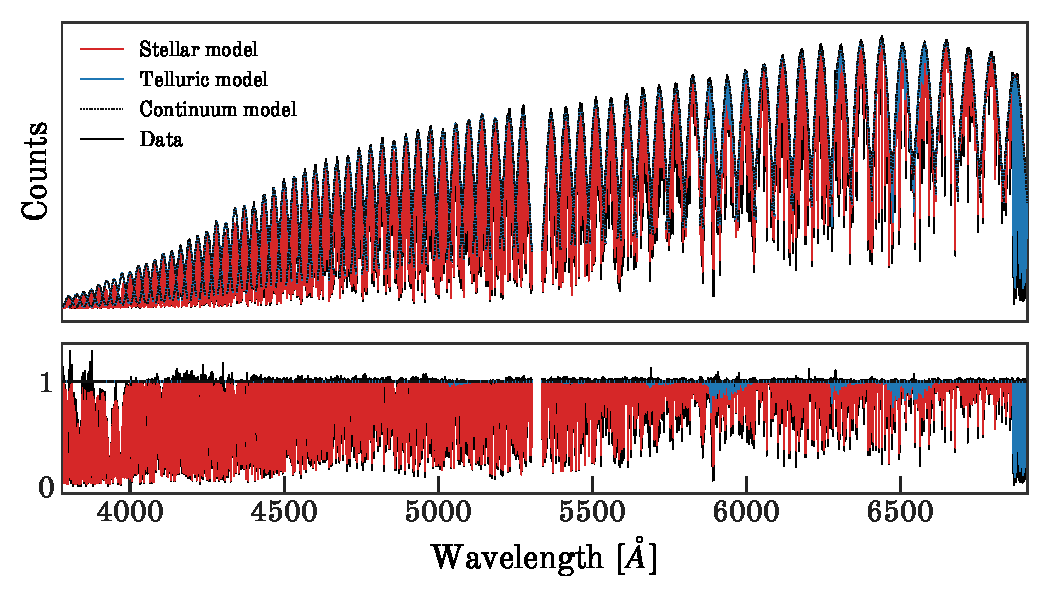
\includegraphics[width=\textwidth]{example.pdf}
    \caption{An example fit to a single \eso/\harps\ spectrum of HD~222595 (black), showing the continuum fits per echelle order (dotted), the stellar absorption model (red) and the telluric transmission model (blue), all fit simultaneously with a constrained linear absorption model. Near the strong Ca H and K lines it is clear that there are \emph{no} `continuum pixels' in those echelle orders, yet the model provides an excellent estimate of the true continuum. \label{fig:example-echelle}}
\end{sidewaysfigure}

The final product of the \harps\ data reduction pipeline is a one-dimensional unrectified spectrum, resampled onto a single wavelength array where all echelle orders have been stitched together. Because we are interested in fitting the continuum on a per-order basis, we instead use the \texttt{e2ds} data products. These are extracted one-dimensional unrectified spectra of each echelle order, with the wavelength solution represented by a low order polynomial. In early experiments we fit the spectra in the \texttt{e2ds} data products directly, an example of which can be seen in Figure~\ref{fig:harps-alf-cen-a}. However, for some exposures we noticed systematic residuals that could be explained by a 2D artefact in the image plane (e.g., a ghost or reflection). While we expect that flat-fielding should have already removed these kinds of artefacts, it did prompt us to explore using the nightly blaze calibration files. Using the calibration blaze files mitigated much of the visible structure, and expectedly \ajw{``as expected'', maybe} provided spectra with a simpler, flatter shape. For these reasons, in all experiments except for the one shown in Figure~\ref{fig:harps-alf-cen-a}, we chose to fit blaze-corrected echelle orders.\\

When fitting each exposure we took the computed Barycentric Earth radial velocity and the radial velocity measured by the \harps\ data reduction pipeline to shift the stellar absorption basis vectors $\vec{F}$ to the observed frame. In situations where no radial velocity was available from the \harps\ data reduction pipeline, we adopted the radial velocity reported by \citep{Someone}. Each exposure has $\sim3\times10^6$ pixels across 72 echelle orders, which we model with 16 stellar basis vectors, 4 telluric vectors, and \todo{9} Fourier modes per echelle order, totalling \todo{668} model parameters per spectrum.\\

We used the same model setup for the second experiment, where we required many spectra taken of the same star at low and high (e.g., 10 to 200) S/N ratios. The lower bound on S/N ratio might be unrealistic since spectroscopists prefer measuring stellar parameters and chemical abundances from higher quality spectra, but the bound is necessary to evaluate performance at low S/N ratios. The \eso/\harps\ catalog revealed that not many stars meet our repeated S/N sampling requirement. When sorted by number of exposures in descending order, $\alpha$-Centauri A was the first star that met our requirements in repeated S/N sampling. We constructed bins of S/N from 0 to 200 in steps of 10, and selected a random $\alpha$-Centauri A spectrum (Table~\ref{tab:obs-alf-cen-a}) for every S/N ratio bin interval to provide an even sampling of spectra at low and high S/N ratios. We fit our model to each spectrum, treating it as totally indepdendent from all others.\\





\begin{figure*}
    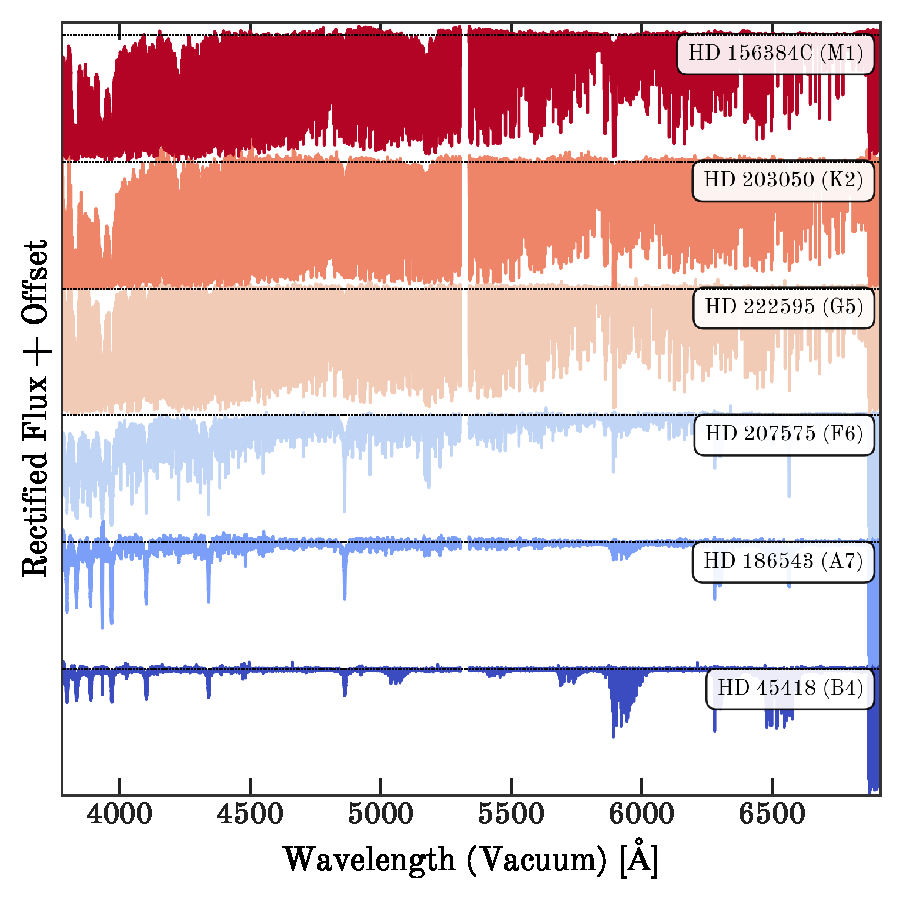
\includegraphics[width=\textwidth, height=\textwidth]{../code/harps_examples.pdf}
    \caption{Continuum-rectified \harps\ spectra of example spectral types from B to M. The model used here includes 16 basis vectors for stellar absorption, and 4 basis vectors for telluric transmission. \todo{Only BAF-type stars used blaze-corrected spectra. Need to download blazes for others and re-run.} \ajw{consider a lower line weight} \ajw{I feel like i'm being thick but I don't get why these ever go above 1. Also, are you sure that the clam continuum is where the theoretical continuum is for the M1 star?}}\label{fig:harps-examples}}
\end{figure*}


\section{Results} \label{sec:results}

We independently fit all \eso/\harps\ spectra referenced in Tables~\ref{tab:harps-examples} and \ref{tab:alf-cen-a}. We found it takes a few core-seconds to fit each exposure. The software implementation released with this paper provides for each echelle order: the predicted flux; the continuum; the rectified model flux; and the telluric transmission. With these we can plot the rectified flux per echelle order, or resample the rectified flux across all echelle orders.\\

The first defined experiment involves fitting stars of a variety of spectral types. The rectified spectra for selected example stars in this experiment are shown in Figure~\ref{fig:harps-examples}, where stars are ordered and coloured by their spectral type listed in \project{SIMBAD}. From these rectified spectra it is clear that the model performs well on a variety of stellar types and evolutionary stages. HD 45418, a B4-type star, is the hottest star in our sample  \citep[$T_\mathrm{eff} = 16{,}750\,K$ according to ][]{2015MNRAS.454...28M}, and far exceeds the upper temperature bound (8,000\,K) of the synthetic grid that we factorized using NMF. The fit to HD 45418 is quite good, despite this star being well outside the model grid. All other example stars shown in Figure~\ref{fig:harps-examples} have literature stellar parameters that place them well within the bounds of the factorized model grid. Most stars observed with \eso/\harps\ are predictably \ajw{drop ``predictably'' maybe} on the main-sequence, since they are more frequently subject to radial velocity exoplanet searches than evolved stars. HD 203050 (K2) is the only red giant branch in our sample. This is not obvious from Figure~\ref{fig:harps-examples}, suggesting the model does just as well on red giant branch stars as it does on main-sequence stars. This has been our experience in other works using this method on SDSS-V optical and near-infrared spectra (Casey et al., in prep).\\


The cooler stars in the example set have almost no so-called `continuum pixels' blueward of 4000\,\AA. This is expected; the continuum estimate provided by the model matches theoretical rectified spectra. It illustrates that the continuum estimate that we fit simultaneously with stellar absorption does provide a closer estimate to the true continuum rather than a pseudo-continuum.\\

There is good agreement between the model fits and data for example stars of different spectral types. In detail there are mis-matches in line absorption strength, or mis-matches in the form of missing lines (in either the model or the data). We discuss model mismatches in Section~\ref{sec:discussion}, but we can surmise that model mis-matches are a result of missing or inaccurate physics in the spectral synthesis code or its inputs (e.g., model atmospheres, line lists, opacities), or due to the poor linear approximation we make for the stellar spectra, or both. In any case, the model appears to be sufficiently accurate to describe the continuum without substantial bias, so it is not a major concern for our purposes. \\

A separate reason for model-data disagreement comes from our use of the telluric transmission model. The telluric models available to us are of lower spectral resolution ($\mathcal{R} \sim 25{,}000$) than \harps. This is apparent when closely comparing the fitted model with the data (e.g., if one could zoom in finely to Figure~\ref{fig:example-echelle}), but it is otherwise not obvious. The model telluric transmission predicts features that are clearly broader than the data, but the telluric basis vectors are a sufficiently good description for the data that the telluric absorption does not get captured by the continuum basis vectors and adversely affect the fit.\\

The second defined experiment tests how consistently we can predict continuum for the same star, as a function of S/N ratio. Given an imperfect (or no) model for stellar spectra, noisy signals can mimic stellar absorption, which causes the continuum to become systematically biased at low S/N ratios. We fit \todo{X} spectra of $\alpha$-Centauri A, which are sampled uniformly in S/N bins from 10 to 200 pixel$^{-1}$. This experiment forces us to select a summary statistic to evaluate the consistency of our continuum rectification. We adopt the 95th percentile in rectified flux as a statistic to compare to normalisation methods described in the literature, but we prefer to view how the \emph{distribution} of normalized flux values change as a function of S/N ratio. Both properties are shown in Figure~\ref{fig:repeatability-with-snr}, where the line indicates the 95th percentile of normalized flux, and the shaded area shows the distribution of normalized flux values. Above S/N $\sim$ 30, both indicators are extremely stable and do not vary significantly with S/N ratio. This is notable, as most spectra acquired for the purpose of stellar parameters and chemical abundances will aim for S/N $>$ 30, but spectra below S/N $<$ 50 are routinely described as being problematic to rectify consistently. From this figure it highlights that we can achieve consistent continuum normalisation whether the star has S/N $\sim$ 30 or 300. \todo{This experiment was done on non-blaze-corrected spectra. I either need to re-do it, or update the text accordingly.}\\

We can make quantitative statements on the consistency of continuum rectification for $\alpha$-Centauri A. Taking the 95th percentile of normalized flux as a proxy statistic for the normalization consistency, we find that above S/N $> 100$, the standard deviation of the 95th percentile of normalized flux is 0.22\%, which is equivalent a spread in normalized flux of 0.0022. This variation is smaller than the typical flux errors, and only increases marginally when we include lower quality spectra. Taking all spectra with S/N $>$ 50, we find the scatter in the 95th percentile of normalized flux to be 0.35\%. With S/N $>$ 30, this rises marginally to 0.46\%. In all scenarios the estimated error in continuum is less than the typical flux error.\\


% alf Cen 95th percentile (all wavelengths)
% for S/N > 100, 1-sigma scatter is 0.22%
% for S/N > 50, 1-sigma scatter is 0.35%
% for S/N > 30, 1-sigma scatter is 0.46%


\begin{figure}
    \includegraphics*[width=\textwidth, height=3in]{alpha-cen-repeat-snr.pdf}
    \caption{Distribution (shaded) of rectified flux of $\alpha$-Centauri A as a function of S/N ratio, with every spectrum fit independently. The line represents the 95th percentile, where the scatter in this percentile is 0.46\% for spectra with S/N $>$ 30, and 0.22\% for everything with S/N $>$ 100. \label{fig:alpha-cen-wrt-snr}}
\end{figure}

\section{Discussion}\label{sec:discussion}

We have shown that a constrained linear model is a good choice for modeling stellar spectra, which enables precise estimates of the continuum for a range of stellar types. Representing stellar absorption using NMF instead of a some other linear representation is particularly advantageous. Non-negativity ensures that stellar basis vectors are strictly additive, and the negative log-transformation we use restricts both the rectified stellar flux and telluric transmission to be between 0 and 1. Any data values outside this range can \emph{only} be captured by the continuum basis vectors. In some sense the predictive capacity of the combination of NMF basis vectors is nearly orthogonal to a combination of the continuum basis vectors.\ajw{Is this a restatement/interpretation of the fact that the stellar line basis and continuum basis are aproximately orthogonal?}\\

NMF is less frequently used in astronomical data analysis than other linear representations. A more common linear representation for this kind of problem is Principal Component Analysis (PCA), which yields an orthogonal decomposition that maximally explains the variance in the data. PCA is made possible by orthogonality, whereas NMF is made possible by the non-negativity constraint. While PCA can capture more variance than NMF for the same data set and number of components, in PCA there are no bounds on the eigenvalues (basis weights). For this reason, if we used PCA to represent stellar spectra then it would make it nearly impossible to determine the continuum. We could model the data without having any continuum basis vectors, simply by finding the first eigenvalue to be a very large positive value, the second eigenvalue to be a large negative value, the third a slightly lower (but still large) positive value, and so on. This can easily model flux values much larger than 1. The situation does not get much better if we include basis vectors for the continuum, because much of that smooth structure can be captured by the PCA spectral model.\\

Another somewhat unexpected advantage to using NMF is that the basis vectors themselves appear to be highly interpretable. For example, one basis vector has only strong hydrogen lines in it. Another only shows molecular CO features that only appear in M-type stars. Another two basis vectors are similar in that they have a forrest of atomic lines, but they vary in the broadness of particularly strong lines (e.g., where one is consistent with pressure broadening in a main-sequence star). General wisdom when working with compressed representations is that the basis vectors should generally be treaated as latent (unobservable) vectors, and there is risk associated with trying to physically interpret them. We avoid physical interpretability here, but in subsequent work we discuss how the basis weights and vectors can be interpreted (Casey et al., in prep). Here we simply reiterate that the stellar parameters used to construct the grid are not used by the NMF process, and the spectra are randomly shuffled during each iteration of factorization, so there is no possible `leakage' of information about effective temperature, surface gravity, metallicity, or other properties. Nevertheless, the resultant basis vectors have absorption features that are strongly correlated with these properties. \\

Chosing not to interpret the basis vectors or weights has specific advantages. For example, if we were to build some mapping from stellar parameters to basis weights, then one could construct a forward model for the data where the model parameters are the continuum coefficients and the stellar parameters (e.g., $T_\mathrm{eff}$, $\log{g}$), instead of continuum coefficients and basis weights. That model would be far less flexible than the model we present here. For example, our model is capable of providing excellent fits to the data, even if the underlying theoretical spectra are inaccurate. A simple example is hydrogen lines. \citep{Wheeler} showed that the hydrogen lines in the infrared are incorrectly computed by many spectral synthesis codes. When we use existing grids with this problem (e.g., like those used in \texttt{FERRE}, as part of \texttt{ASPCAP}), if we had a model that was mapping from stellar parameters to basis weights, then even if the hydrogen lines are in their own basis vector, we would find a biased estimate of effective temperature, or a worse fit to the data, or both. Instead, by not restricting ourselves to a mapping between stellar parameters to basis weights, we retain flexibility to make excellent fits to the data.\\



Our model is limited by how well it predicts data in two different ways. The first is in how well the models of stellar atmospheres, line lists, and spectral synthesis codes can match real data. There is very little we can do about that error mis-match here. The second form of error arises in our factorization of the grid. We could add more basis vectors, train for longer, even include estimated per-pixel model uncertainties, but the reconstruction will never be perfect. A related minor deficiency in our model choice is that it cannot model emission lines in stellar spectra: the model can only predict rectified flux values between zero and one. This is a minor problem because emission lines are rare, only occurring in the strongest of lines for chromospherically active stars, and because the emission lines only affect a small number of pixels, they contribute very little to the overall $\chi^2$.\\

The speed of our model makes it particularly advantageous for evaluating on large data sets. If we assume that the factorization of stellar spectra introduces a small error relative to the usual mis-match between models and data, then a constrained linear model represents a promising avenue for identifying regions where models and observations disagree the most. The simplest path for doing this might be to look at the total squared residuals as a function of pixel across many stars, which would immediately indicate the areas where the model does not have capacity to predict the data. Next steps might be to improve modelling for that region (e.g., through better line lists) or might be to iteratively update the basis vectors in a data-driven way so that they better match the data. The model is trained from synthetic spectra, so it is already a close approximation to what stellar spectra look like, and doing data-driven updates would be an excellent way to handle severe data-model mis-matches (e.g., large molecular features which are present in data but we lack line lists to accuratley model). There is a lot of flexibility when updating the basis vectors using multiplicative update rules: we can restrict ourselves to only allowing updates on particular pixels (where there is sharp disagreement), and we can restrict ourselves to only updating a single basis vector. \ajw{a reader might be puzzled by the claim that you can evaluate the goodness of the model spectra given the discussion above about how it's fine if the model spectra are a bit shit.}\\

%We have demonstrated the effectiveness of a constrained linear absorption model for continuum normalization across a range of spectral types. 

There are not many literature metrics to choose from when evaluating performance of continuum normalization. We have qualitatively shown the distribution of rectified flux values for $\alpha$-Centauri A, and quantitatively estimated the precision from the scatter in the 95th percentile of rectified flux values. These statistics are computed using all wavelengths, but it is well-known that continuum is easier to model at redder optical wavelengths because there are fewer absorption features. One excellent examination of continuum normalization consistency is that of \citet{RASSINE}, where they report consistent continuum normalization at the level of 2\% based on applications to extremely high quality ($S/N > 1000$) \eso/\harps\ spectra of $\alpha$-Centauri B stacked over consecutive nights, and 0.29\% for a comparably high quality spectrum of the Sun. Their statistic is defined as the 2$\sigma$ of $1-f_i$, where $f_i$ is the $i$th normalized flux value at the anchor point locations used to build the continuum. The anchor points are chosen by the user, which makes for a less direct comparison with our statistic, but for these purposes we will assume that the continuum anchor points are perfectly chosen and truely represent the continuum in the star. Given these assumptions, for comparison purposes we take \texttt{RASSINE} as providing 1\% consistency in continuum estimates for S/N $> 1000$ spectra of $\alpha$-Centauri B, and 0.15\% consitency for comparable Solar spectra. If they restrict their statistic to wavelengths redder than 4500\,\AA, their precision for $\alpha$-Centauri B improves to 0.6\%. In comparison, for spectra we use that is 1/10th the S/N ratio, we find our method yields consistent continuum estimates at the level of 0.22\%.\\

%\todo{I really don't want to, but should I Fisher information matrix and predict how precisely we could estimate the continuum as a function of S/N for this model? It's linear so it's simple, but it adds necessitates a lot of explanatory text that is not easily digestible by my target audience (spectroscopists).}\\

%\citet{Someone} also describes an estimate of the line depth precision achieved using \texttt{RASSINE}. Their estimates of line depth precision outperform (by percentage) their continuum estimates. 
%\todo{RASSINE talk about line depth precision and i dont know if i want to get into that. if line depth precision is good but the continuum precision is bad then it doens't really matter what you line depth precision is because it will be dominated by the continuum accuracy in that we measure line depths relative to the continuum}

Arguments on the consistency of continuum normalization are precision-based arguments, which says nothing about accuracy. That is unfortunate for us because any pseudo-continuum method explicitly only needs to make arguments about precision: a pseudo-continuum is not intended to be accurate! In our case, our model is built to try and estimate the true continuum as best as possible by properly accounting for the stellar absorption. While this does likely lead to a more accurate estimate of the continuum, measuring that accuracy is very hard. Getting the continuum absolutely correct requires a stellar spectrum of a flux-calibrated instrument, and it requires that we have good models of stellar absorption. Some instruments deliver flux-calibrated spectra, but we rarely believe that we have good models of stellar absorption for M-type stars. Here, we think we do have good models of stellar absorption for M-type stars, but there are known deficiencies: the CaH and TiO bands are poorly modelled in most synthetic spectral grids, including the one we used. %If we think we have a good fit to data from a flux-calibrated instrument such that we believe we have an accurate measure of the continuum, how would we independently test that accuracy? If the star was a standard candle, in that we knew how bright it should appear at a given distance, and we used the geometric parallax to get a distance, then we could state what the expected flux should be and compare that with our estimate of the continuum. But M-dwarf stars are not standard candles. 
Put simply, measuring accuracy of continuum is hard, and we don't try it, but we think our continuum estimate is better than a pseudo-continum.\\

We used the radial velocities reported by the \eso/\harps\ pipeline to shift stellar basis vectors to the observed frame. In cases of extreme rotational broadening, we also used literature measures of $v\sin{i}$. We took both of these quantities as truth, but in fact we could fit for them simultaneously. A radial velocity shift and a convolution are both linear operators, in that they can be incorporated in our model without breaking our strict linearity constraint. We would have to change how we solve the system: we could no longer solve the system directly by unconstrained least-squares, or with the truncated reflective region algorithm, but we would have to solve it using linear operators that output the dot product and left adjoint transpose dot product. Alternatively, given the speed of our model, one could imagine a grid in radial velocities (e.g., in $\pm1\,000\,\mathrm{km}\,s^{-1}$), where at each radial velocity we solve for $\vec{\tilde{X}}$ and then take the radial velocity with the lowest $\chi^2$. This is a robust method that has been used for decades. The rotational broadening can be estimated from the cross-correlation in the same way. For these reasons, the method we describe here is readily extensible to situations where the radial velocity and the rotational broadening is not known.\\


\section{Conclusions} \label{sec:conclusions}

We introduce a novel approach to modelling stellar spectra as a linear combination of highly constrained absorption vectors, which we show is sufficient for simultaneously fitting stellar absorption, telluric transmission, and the joint continuum-instrument response. A constrained linear absorption model has many advantagous properties over alternative data-driven methods or machine learning techniques used in stellar spectroscopy. The model structure restricts basis vectors to be strictly additive, ensuring separability between the basis vectors for absorption and continuum. The model requires no initial guess or prior of the stellar parameters, and the linearity ensures that inference is robust, stable, and fast. An extension of this work could also solve for other linear nuisances (e.g., radial velocity, rotational broadening). Finally, an unexpected result of this work is that the basis vectors found from factorizing model rectified spectra appear to be highly interpretable, which is promising for their use for interpretable constrained linear absorption models.\\

%Basis vectors learned by factorizing rectified grids of stellar spectra separate out into vectors that include only hydrogen lines, atomic lines, or prominent molecular features. A specific example of interpretability is shown where ony basis vector incldues only strong hydrogen lines, and at inference time we find the corresponding weight for this vector increases smoothly with spectral type (a proxy for effective temperature). 

%- data-driven stuff with model specification, more flexible than it needs to be, and then there are things taht model stuff as abosrption like blaze, Ella Wang bright-oblique method,


%\noindent{}We provide a Python implementation of our method in the following repository: \url{https://github.com/andycasey/continuum}.

\paragraph{Software}
\texttt{numpy} \citep{numpy}; 
\texttt{matplotlib} \citep{matplotlib}; 
\texttt{scipy} \citep{scipy};
\texttt{scikit-learn} \citep{scikit_learn}.


\paragraph{Acknowledgements}
If they do not become co-authors, then we should be sure to thank
    Jon Holztman (NMSU),
    Rory Smith (Monash),
    Adam Wheeler (CCA),
    Andrew Saydjari (Harvard),
    Guy Stringfellow,
    Lily Zhao (Chicago),
    Julianne Dalcanton (CCA),
    David W. Hogg (NYU),
    Megan Bedell (CCA), and
    Michael Blanton (NYU).

\todo{Acknowledge Utah and OzStar resources. Acknowledge NYU for accommodating my body as it withered without free Flatiron lunch.}
% include bibliography
\bibliographystyle{aasjournal}
%\bibliography{bibliography}

\end{document}
